\documentclass[aspectratio=169, 8pt, xcolor={svgnames}, hyperref={linkcolor=black}]{beamer}
\setbeamercolor{background canvas}{bg=white}

\usepackage[labelfont={color=amethyst,bf}]{caption}
\usetheme[progressbar=frametitle]{metropolis}
\usepackage{appendixnumberbeamer}
\usepackage{url}
\usepackage{booktabs}
\usepackage{braket}
\usepackage[scale=2]{ccicons}
\usepackage{amsfonts}
\usepackage{amssymb}
\usepackage[english]{babel}
\colorlet{col1}{teal}
\colorlet{col2}{yellow}
\colorlet{col3}{green}
\usepackage{fontawesome}
\usepackage{multicol}
\usepackage{bm}
\usepackage{algorithm}
\usepackage{algpseudocode}
\usepackage{enumitem}

\usepackage[]{pseudo}


\usepackage{tikz}
\usetikzlibrary{positioning,arrows,calc,math,angles,quotes}
\usepackage{blochsphere}

\usetikzlibrary{arrows,automata}
\usetikzlibrary{positioning}
\usetikzlibrary{arrows.meta,
                bending,
                intersections,
                quotes,
                shapes.geometric}

\tikzset{
    state/.style={
           rectangle,
           rounded corners,
           draw=black, very thick,
           minimum height=1em,
           inner sep=2pt,
           text centered,
           },
}


\definecolor{myv}{rgb}{0.36, 0.22, 0.33}
\definecolor{gio}{rgb}{0.45, 0.31, 0.59}
\definecolor{light}{rgb}{0.8, 0.8, 1}
\definecolor{warmblack}{rgb}{0.0, 0.26, 0.26}
\definecolor{brown(web)}{rgb}{0.65, 0.16, 0.16}
\definecolor{cadmiumgreen}{rgb}{0.0, 0.42, 0.24}
\definecolor{darkmidnightblue}{rgb}{0.0, 0.2, 0.4}
\definecolor{brightube}{rgb}{0.82, 0.62, 0.91}

\definecolor{codegreen}{rgb}{0,0.6,0}
\definecolor{codegray}{rgb}{0.5,0.5,0.5}
\definecolor{codepurple}{rgb}{0.58,0,0.82}
\definecolor{backcolour}{rgb}{0.95,0.95,0.92}
\definecolor{amethyst}{rgb}{0.6, 0.4, 0.8}

\definecolor{light-gray}{gray}{0.95}
\newcommand{\code}[1]{\colorbox{light-gray}{\texttt{#1}}}

\usepackage{listings}
\lstdefinestyle{mystyle}{
    backgroundcolor=\color{backcolour},
    commentstyle=\color{codegreen},
    keywordstyle=\color{codepurple},
    numberstyle=\tiny\color{codepurple},
    stringstyle=\color{magenta},
    basicstyle=\scriptsize,
    breakatwhitespace=false,
    breaklines=true,
    captionpos=b,
    keepspaces=true,
    numbers=left,
    numbersep=5pt,
    showspaces=false,
    showstringspaces=false,
    showtabs=false,
    tabsize=2
}

\lstset{style=mystyle}
\usepackage[most]{tcolorbox}
\usepackage{xcolor}

%\usepackage[citecolor = green, linkcolor = blue, bookmarks=true, urlcolor=blue,
%colorlinks=true, pagebackref=true]{hyperref}



%\usepackage{xspace}

\title{A few slides on full-stack QML}



\begin{document}

\begin{frame}
\maketitle
\end{frame}

\begin{frame}{Quantum Machine Learning challenges}
We aim to involve quantum process units into Machine Learning pipelines.
\begin{figure}
   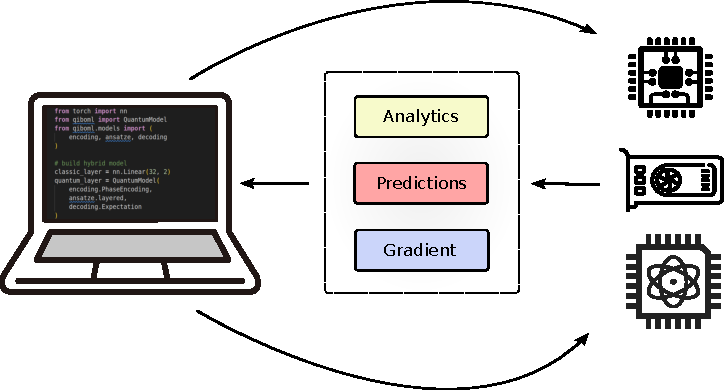
\includegraphics[width=0.7\textwidth]{figures/hybrid.pdf}
\end{figure}
Classical and quantum components have to be executable on CPUs, GPUs and QPUs to
fullfill the whole potential of an hybrid quantum-classical cluster.
\end{frame}

\begin{frame}{Qibo as a modular playground}
To do so, \texttt{Qibo} stands as an intriguing playgrond thanks to its modularity.

Once a favourite ML framework is chosen, a quantum circuit can be built with Qibo
and included into the pipeline. 
\begin{figure}
   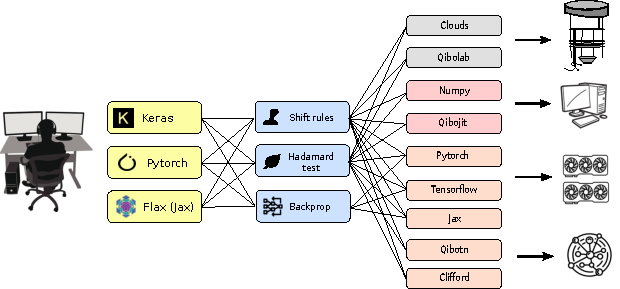
\includegraphics[width=0.7\textwidth]{figures/qiboml_nn_2.pdf}
\end{figure}
The circuit can then be executed onto the desired Qibo backend (quantum or classical).
\end{frame}

\begin{frame}{A practical example of an hybrid quantum-classical pipeline with \texttt{Qibo}}
We want to learn the Parton Distribution Function of the $up$ quark in the proton with a superconducting qubit.

In doing so, we want to mitigate the noise of the quantum device using a learning-based error mitigation technique.

\begin{multicols}{2}
The method requires:
\begin{itemize}[noitemsep]
\item[1.] efficient classical simulation tools;
\item[2.] easy access to the quantum hardware;
\item[3.] ability to easily make quantum and classical outputs interact;
\item[4.] access to GPUs clusters if the process is part of a ML pipeline (optionally). 
\end{itemize}
\begin{figure}
   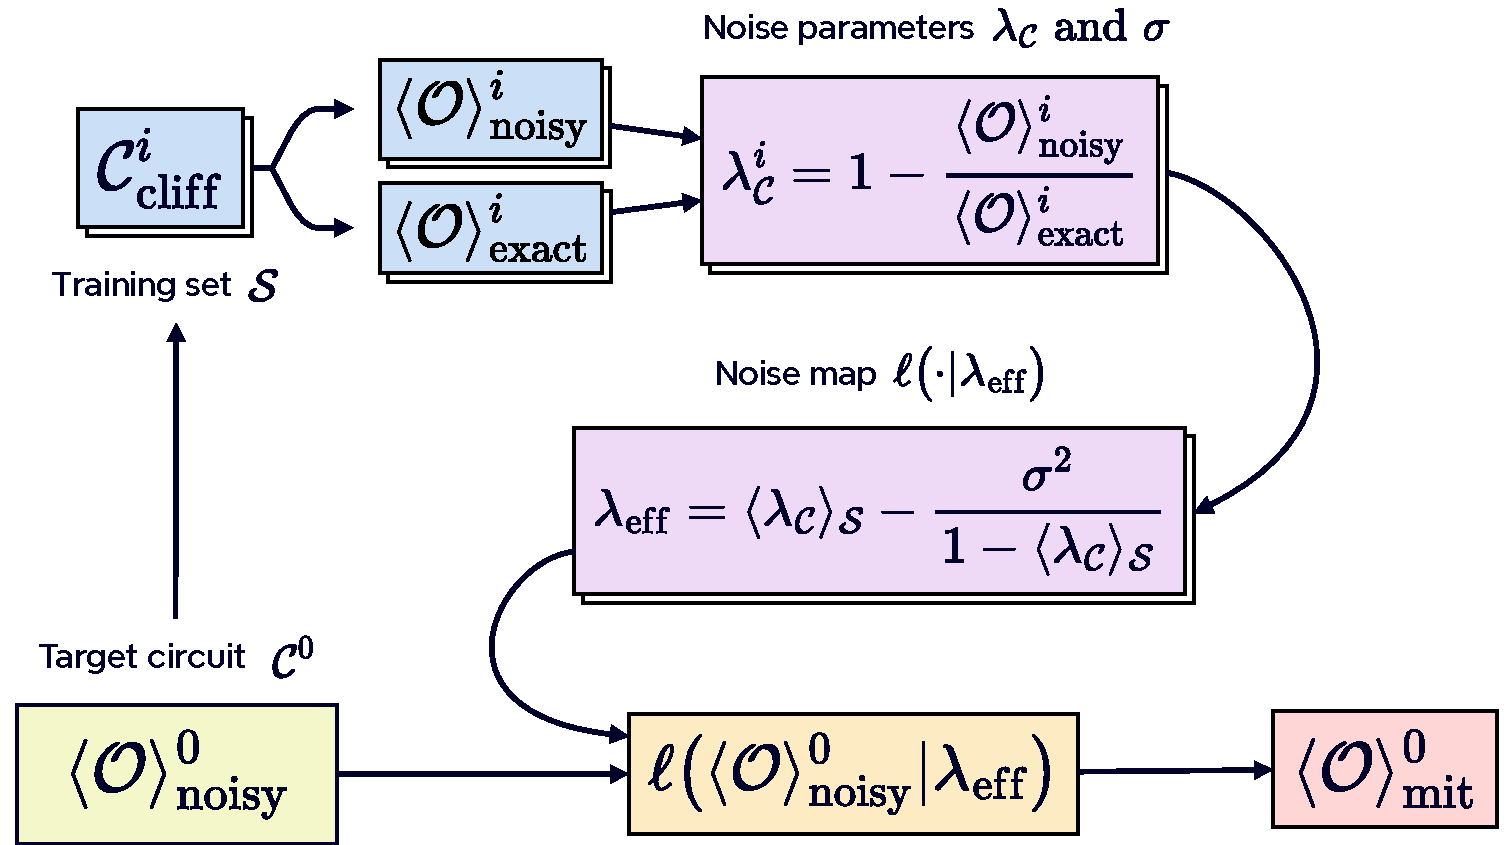
\includegraphics[width=0.5\textwidth]{figures/ics.pdf}
\end{figure}
\end{multicols}
\end{frame}

\begin{frame}{PDF fit on chip \hfill \faBook\,\, \href{https://arxiv.org/abs/2308.06313}{arXiv:2308.06313}}

\begin{multicols}{2}
% column 1
\hspace{2cm}
\begin{tcolorbox}[title=High level API: Qibo, colback=blue!20]
\begin{itemize}[noitemsep]
\small
   \item[\faCode] define \textbf{prototypes} and models;
   \item[\faCode] \textbf{simulate} training and noise.
\end{itemize}
\end{tcolorbox}
\begin{tcolorbox}[title=Calibration: Qibocal, colback=yellow!20]
\begin{itemize}[noitemsep]
\small
   \item[\faCrosshairs] \textbf{calibrate} qubits;
   \item[\faCrosshairs] generate \textbf{platform configuration};
\end{itemize}
\end{tcolorbox}
\begin{tcolorbox}[title=Execution: Qibolab, colback=red!20]
\begin{itemize}[noitemsep]
\small
   \item[\faCog] allocate \textbf{calibrated} platform;
   \item[\faCog] \textbf{compile} and \textbf{transpile} circuits;
   \item[\faCog] execute and return \textbf{results}.
\end{itemize}
\end{tcolorbox}
% column 2
% PDF image
\begin{figure}  
    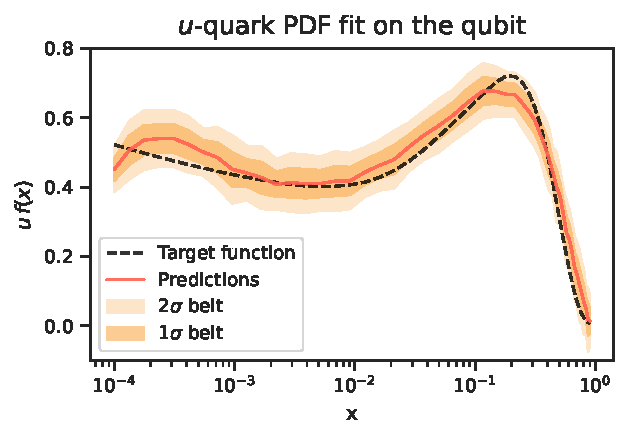
\includegraphics[width=0.38\textwidth]{figures/qpdf.pdf}
\end{figure}
% parameters
\begin{center}
\begin{table}
\vspace{-0.5cm}
\begin{tabular}{cc}
\hline \hline 
\textbf{Parameter} & \textbf{Value} \\
\hline 
$N_{\rm data}$ & 50 \\
$N_{\rm shots}$ & 500 \\
MSE & $\sim 10^{-3}$ \\
Electronics & Xilinx ZCU216 \\
Training time & $\sim 2$h \\
\hline \hline
\end{tabular}
\end{table}
\end{center}
\vspace{0.5cm}
\end{multicols}
\begin{picture}(0,0)
    \put(355,75){
        
\includegraphics[width=0.12\textwidth]{figures/homemade.png}
    }
\end{picture}
\end{frame}

\begin{frame}{Real-time quantum error mitigation}
We define a Real-Time Quantum Error Mitigation (RTQEM) procedure.
\begin{figure}
    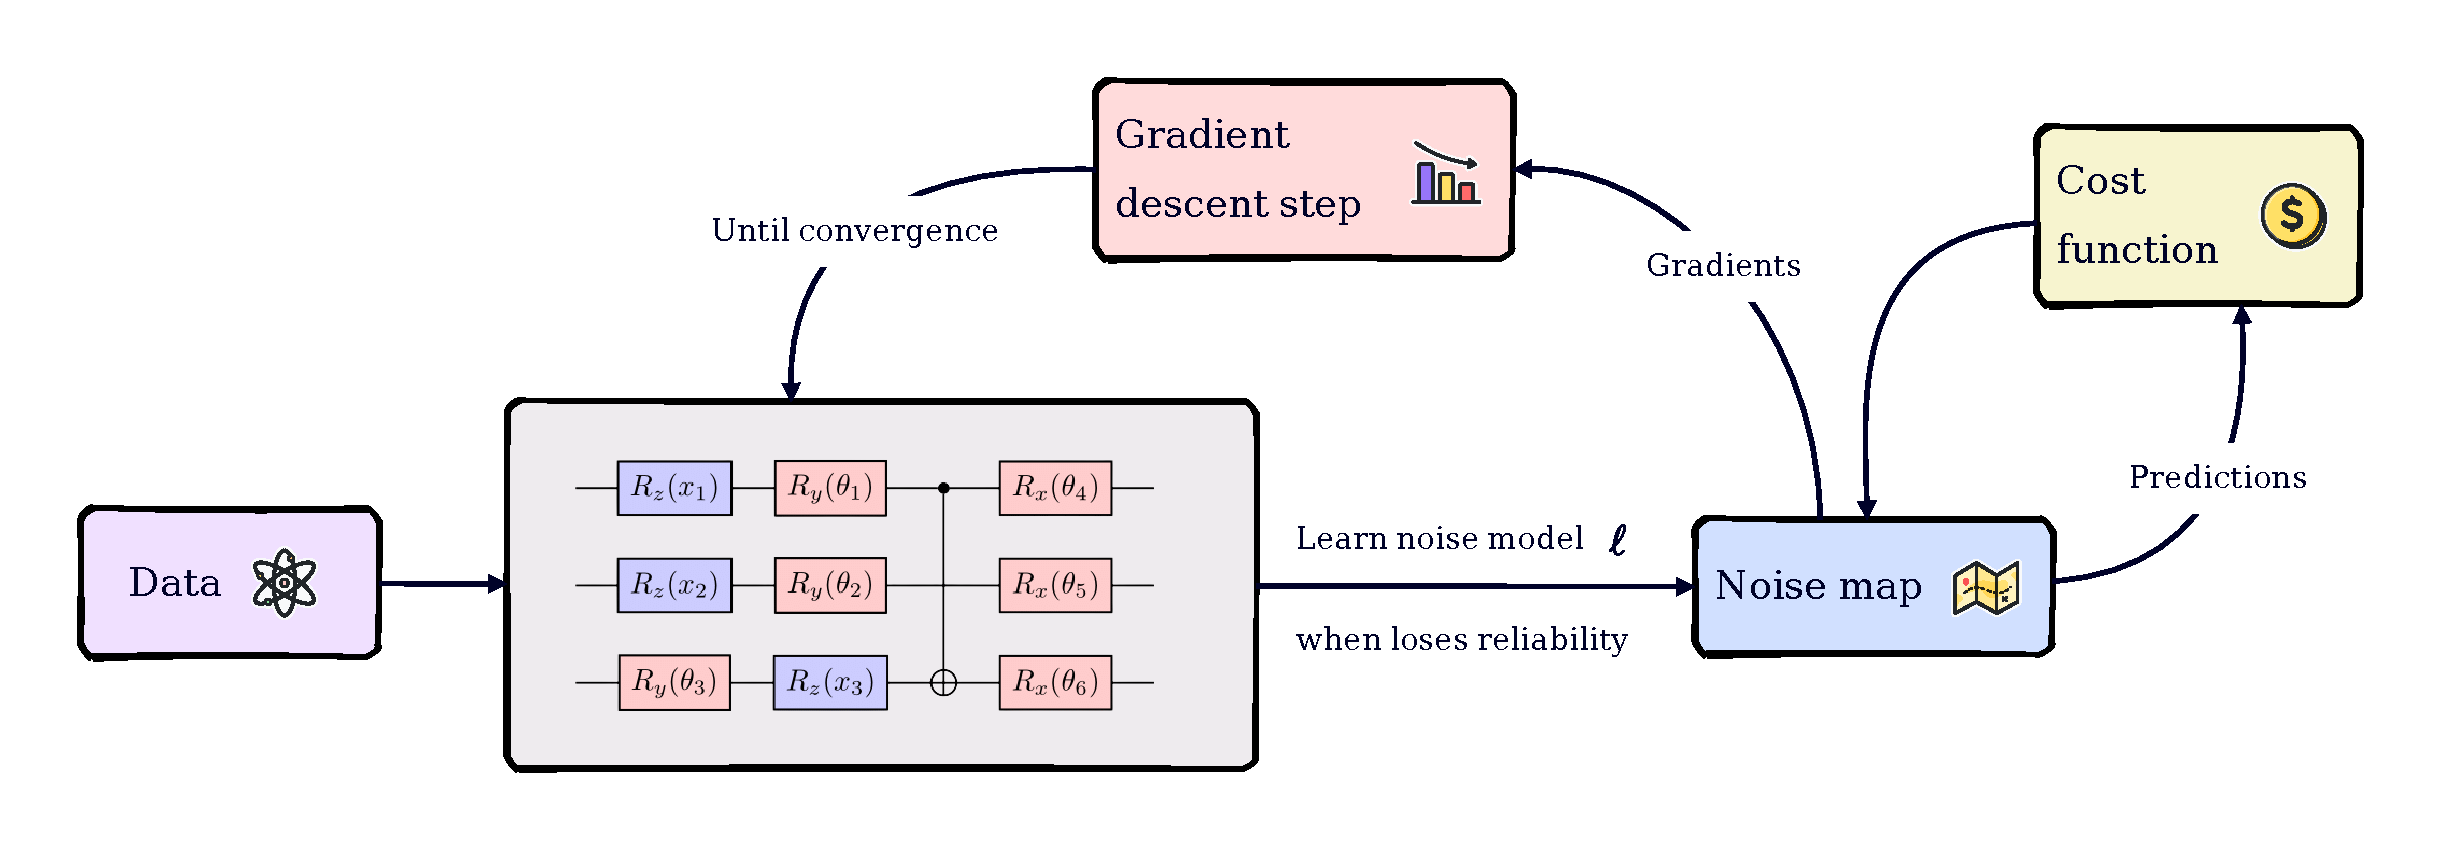
\includegraphics[width=0.8\textwidth]{figures/rtqem.pdf}
\end{figure}
\begin{itemize}[noitemsep]
\item[1.] consider a Variational Quantum Algorithm trained with gradient descent;
\item[2.] learn the noise map $\ell$ every time is needed over the procedure;
\item[3.] use $\ell$ to clean up both predictions and gradients.
\end{itemize}
This procedure requires real-time interaction between quantum and classical devices:
the former returns the output of the quantum system, the latter mitigate the noise.
\end{frame}

\begin{frame}{RTQEM in action}
We perform a gradient descent on two different quantum devices (and noises!)
\begin{center}
\begin{tabular}{cccccc}
\hline \hline 
\rule{0pt}{2.5ex}
\textbf{Parameter} & $N_{\rm train}$ & $N_{\rm params}$ & $N_{\rm shots}$ & Epochs \\
\hline
\rule{0pt}{2.5ex}
\textbf{Value} & $15$ & $16$ & $500$ & $100$ \\
\hline \hline 
\end{tabular}
\end{center}
\begin{multicols}{2}

\begin{figure}
    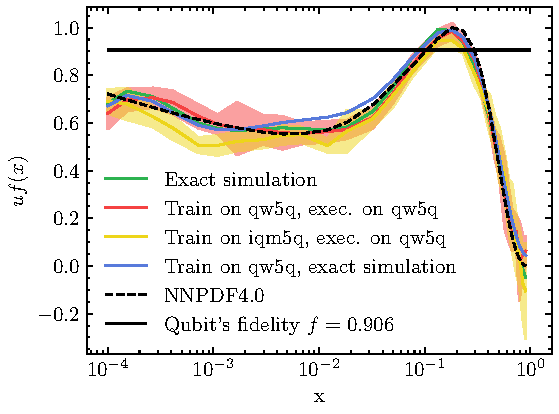
\includegraphics[width=0.4\textwidth]{figures/100.pdf}%
\end{figure}
\begin{center}
\begin{itemize}[noitemsep]
  \item[\faCog] \textbf{\texttt{qw5q}} from QuantWare and controlled using Qblox instruments;
  \item[\faCog] \textbf{\texttt{iqm5q}} from IQM and controlled using Zurich Instruments.
\end{itemize}
\footnotesize
\begin{table}
\begin{tabular}{ccccc}
\hline \hline 
\textbf{Train.} & \textbf{Epochs} & \textbf{Pred.} &  \textbf{Config.} & MSE \\
\hline    
\texttt{qw5q} & 100 & \texttt{qw5q} & RTQEM & $0.0013$  \\     
\texttt{iqm5q} & 100 & \texttt{qw5q} & RTQEM & $0.0037$ \\   
\texttt{qw5q} & 100& \texttt{sim} & RTQEM & $0.0016$ \\   
\hline \hline
\end{tabular}
\centering
\end{table}
\end{center}
\end{multicols}
All the hardware results are obtained deploying the $\bm{\theta}_{\rm best}$ on 
\texttt{qw5q}.
\end{frame}

\end{document}




